\documentclass[12pt, a4paper, twoside, openright, english]{book}

\usepackage[english]{babel}
\usepackage[utf8]{inputenc}
\usepackage[T1]{fontenc}
\usepackage[top=2.5cm,
	bottom=3cm,
	right=3.2cm,
	left=3.2cm
]{geometry}

\usepackage{subcaption}
\usepackage{hyperref}
\usepackage{enumitem}
\usepackage{tabularx}
\usepackage{afterpage}
\usepackage{longtable}
\usepackage{multirow}
\usepackage{amsfonts}
\usepackage{amssymb}
\usepackage{listings}
\usepackage{titlesec}
\usepackage{setspace}
\usepackage{fancyhdr}
\usepackage{fancyvrb}
\usepackage[fleqn]{amsmath}
\usepackage{pdfpages}
\usepackage{nccmath}
\usepackage{tocloft}
\usepackage{csquotes}
\usepackage{diagbox}
\usepackage{ifthen}
\usepackage{algorithm}
\usepackage{algpseudocode}
\usepackage[super]{nth}

\usepackage{colortbl}
\usepackage{tabulary}
\usepackage{adjustbox}


\usepackage{nomencl}
\usepackage{makeidx}
\usepackage{expl3}
\usepackage{etoolbox}
%\preto\tabular{\shorthandoff{-}}

\usepackage[style=iso-numeric, backend=biber]{biblatex}
\addbibresource{literature.bib}

% Zoznam skratiek
\makenomenclature
%\renewcommand{\nomname}{Zoznam skratiek a pojmov}

% Algoritmy
\makeatletter
\renewcommand*{\ALG@name}{Algorithms}
%\renewcommand{\listalgorithmname}{Zoznam algoritmov}
\algrenewcommand\algorithmicrequire{\textbf{Input:}}
\algrenewcommand\algorithmicensure{\textbf{Output:}}
\makeatother

% Empty even pages at the end of chapter
\makeatletter
\renewcommand*{\cleardoublepage}{\clearpage\if@twoside \ifodd\c@page\else
\hbox{}%
\thispagestyle{empty}%
\newpage%
\if@twocolumn\hbox{}\newpage\fi\fi\fi}
\makeatother


% Číslo kapitoly na rovnakom riadku ako názov
\titleformat{\chapter}{\normalfont\huge\bf}{\thechapter}{1em}{}

\raggedbottom
\newcommand{\emptypage}{\newpage\thispagestyle{empty}\mbox{}\newpage}
\newcommand{\signaturespace}[2]{
  \begingroup
  \renewcommand{\arraystretch}{0}
  \begin{tabular}[t]{cc}
  \hspace*{0pt}
  \cleaders\hbox{\kern.6pt.\kern.6pt}\hskip#1\relax
  \hspace*{0pt}
  \\[0.5cm]
  #2
  \end{tabular}
  \endgroup
}

\pagestyle{fancy}
\fancyhf{}  % clear all header and footers
\fancyhead[LE]{\leftmark}
\fancyhead[RO]{\rightmark}
\fancyfoot[LE, RO]{\thepage}

\fancypagestyle{plain}{
  \fancyhf{}
  \renewcommand{\headrulewidth}{0pt}
  \fancyhf[lef,rof]{\thepage}
}

\setlength{\headheight}{16pt}

\renewcommand{\ttdefault}{pcr}
\lstdefinestyle{cstyle}{
    language=C,
	basicstyle=\linespread{1.1}\ttfamily\footnotesize,
    numbers=left,
    numberstyle=\tiny,
    frame=single,
    tabsize=4,
    captionpos=b,
    breaklines=true,
    texcl=true,
	numbersep=8pt,
	framexleftmargin=15pt,
	xleftmargin=5ex,
    xrightmargin=3.4pt,
	morekeywords = {uint8_t,uint16_t,int16_t,uint32_t,int32_t,bool}
}
\lstdefinestyle{docs}{
    language=C,
	basicstyle=\linespread{1.1}\ttfamily\small\bfseries,
    tabsize=4,
    breaklines=true,
    belowskip=0pt
}
\renewcommand{\lstlistingname}{Source code}

\setstretch{1.5}
\newcommand{\University}[0] {Slovenská technická univerzita v Bratislave}
\newcommand{\UniversityEN}[0] {Slovak University of Technology in Bratislava}
\newcommand{\Faculty}[0] {Fakulta informatiky a informačných technológií}
\newcommand{\FacultyEN}[0] {Faculty of Informatics and Information Technologies}
\newcommand{\Thesis}[0] {Diplomová práca}
\newcommand{\ThesisEN}[0] {Master's Thesis}
\newcommand{\Title}[0] {Vibrodiagnostika strojov s~priemyselným internetom vecí}
\newcommand{\TitleEN}[0] {Machinery vibrodiagnostics with the~industrial internet of things}
\newcommand{\Author}[0] {Bc. Miroslav Hájek}
\newcommand{\Supervisor}[0] {Ing. Marcel Baláž, PhD.}
\newcommand{\DepartmentalAdvisor}[0] {Ing. Jakub Findura}
\newcommand{\Consultant}[0] {Ing. Lukáš Doubravský}
\newcommand{\SupervisorEN}[0] {Dr. Marcel Baláž}
\newcommand{\RegNo}[0] {FIIT-xxxx-xxxxxx}
\newcommand{\Date}[0] {Máj 2022}
\newcommand{\DateEN}[0] {May 2023}
\newcommand{\StudyProgramme}[0] {Inteligentné softvérové systémy}
\newcommand{\StudyProgrammeEN}[0] {Intelligent Software Systems}
\newcommand{\StudyField}[0] {Informatika}
\newcommand{\StudyFieldEN}[0] {Informatics}
\newcommand{\Institute}[0] {Institute of Computer Engineering and Applied Informatics}
\newcommand{\SignPlace}[0] {Bratislava, }
\newcommand{\SignDateEN}[0] {May 2023}


\begin{document}
\nomenclature{\textbf{Pojem}}{Vysvetlenie}
% Obal -----------------------------------------------------------------------
\thispagestyle{empty}
{\centering
	{\Large \UniversityEN}\par
	{\Large \FacultyEN}\par
	\vspace{\medskipamount}
	\RegNo
	\vfill
	\textbf{\Large \Author}\par
	\vspace{1.5\bigskipamount}
	\textbf{\LARGE \TitleEN}\par
	\vspace{1.5\bigskipamount}
	{\Large \ThesisEN}\par
	\vfill
}
\begin{flushleft}

{\large Thesis Supervisor: \Supervisor \\
\DateEN}
\end{flushleft}
\emptypage

%  Hlavná časť -----------------------------------------------------------------------
\newgeometry{top=2.5cm, bottom=3cm, right=2.5cm, left=3.5cm}

% Titulný list
\pagenumbering{roman}
\thispagestyle{empty}
{\centering
	{\Large \UniversityEN}\par
	{\Large \FacultyEN}\par
	\vspace{\medskipamount}
	Reg. No. \RegNo
	\vfill
	\textbf{\Large \Author}\par
	\vspace{1.5\bigskipamount}
	\textbf{\LARGE \TitleEN}\par
	\vspace{1.5\bigskipamount}
	{\Large \ThesisEN}\par
	\vfill
}
\begin{flushleft}
\begin{longtable}[l]{ll}
Study programme: & \StudyProgrammeEN \\
Study field: & \StudyFieldEN \\
Training workplace: & \Institute\\
Thesis supervisor: & \Supervisor \\
Departmental advisor: & \DepartmentalAdvisor \\
Consultant: & \Consultant \\
\end{longtable}
\indent\DateEN
\end{flushleft}
\emptypage

% Zadanie
\thispagestyle{empty}
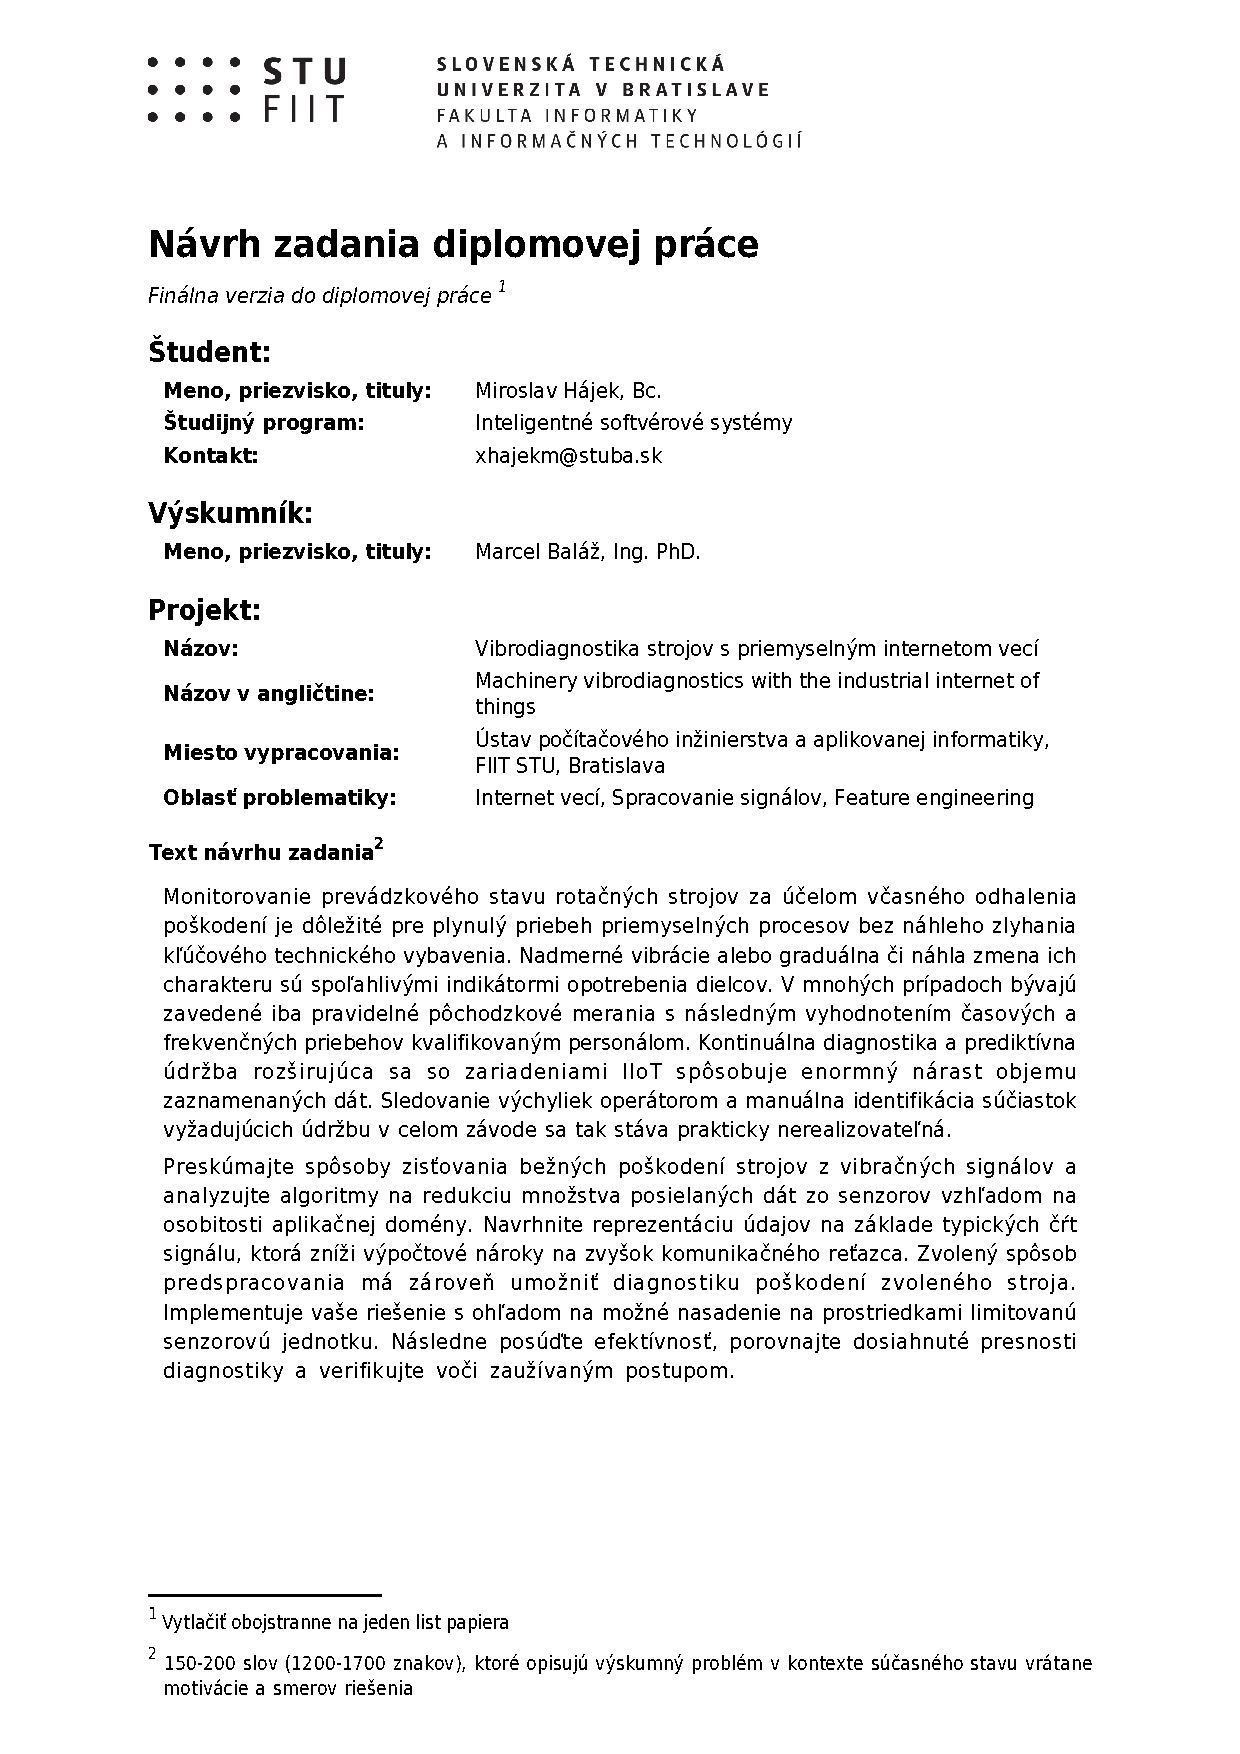
\includepdf[pages=-, scale=1]{chapters/assignment}
\emptypage

 % Declation of Honour
\thispagestyle{empty}
\vspace*{\fill}
\section*{Declation of Honour}

I hereby declare on my honour that I wrote this thesis independently under supervision of Dr. Marcel Baláž, after consultations and with use of cited literature.

\vspace{3\medskipamount}\noindent
\SignPlace \SignDateEN \hspace*{\fill} \signaturespace{5cm}{\Author} 

\emptypage
% Poďakovanie
\thispagestyle{empty}
\vspace*{\fill}
\section*{Acknowledgement}

\vspace{3cm}
\emptypage
\thispagestyle{empty}
\section*{Annotation}
\UniversityEN \\
\uppercase{\FacultyEN}
\vspace{-8pt}
{\setlength{\mathindent}{0cm}
\begin{align*}
&\text{Degree course:} && \text{\StudyProgrammeEN} \\
&\text{Author:} && \text{\Author} \\
&\text{\ThesisEN:} && \text{\TitleEN} \\
&\text{Supervisor:} && \text{\SupervisorEN} \\
&\text{\DateEN}
\end{align*}}

\emptypage 

\thispagestyle{empty}
\section*{Anotácia}
\University \\
\uppercase{\Faculty}
\vspace{-8pt}
{\setlength{\mathindent}{0cm}
\begin{align*}
&\text{Študijný program:} && \text{\StudyProgramme} \\
&\text{Autor:} && \text{\Author} \\
&\text{\Thesis:} && \text{\Title} \\
&\text{Vedúci diplomovej práce:} && \text{\Supervisor} \\
&\text{\Date}
\end{align*}}

\emptypage

% Obsah
\pagestyle{empty}
\tableofcontents{}
\listoffigures
{\let\clearpage\relax \printnomenclature}
\emptypage

\pagestyle{fancy}
% Kapitoly
\pagenumbering{arabic}

\chapter{Introduction}
Manufacturing is experiencing a shift in the traditional practices of asset operational status evaluation and utilization. The rise of Industry 4.0 means greater automation and robotization of the production halls to achieve optimal usage of available resources. The secondary aspect in the enterprises' endeavor, however not less important, is to keep track of the equipment wear and tear. The corrective action be it repair or replacement should be taken on time in response to the key indicators. 

The goal is to preserve required safety and production efficiency when extending the useful life of machine moving parts. In the factories and logistics where this sort of equipment is vital, there is a rising interest in the ability to monitor in real-time the health of the machines and to proactively diagnose the fault to repair it without adding unnecessary costs. 

Vibrations are the most nonintrusive way with which such faults can be sensed. The experts use it to distinguish faulty states and to identify the malfunction's root cause. In critical circumstances such as in the case of the large turbines in the power plants, the precautions leading to regular machinery check-ups are already in place. To reach wider acceptance and spread, the monitoring solution has to be sufficiently independent, reliable, and as self-sufficient as the model design allows it to be.

The main issue to consider in large-scale machinery monitoring using vibrations are lots of uninformative streams of samples not directly useful for the production line operator. The dashboard must aggregate these flows into trend variables with severity levels categorized based on industrial standards. The majority of signals are viewed once at the maximum therefore to store or even transmit them from the edge device in its entirety would be wasteful. The complex overview of the mechanical equipment status is attainable only when agent devices and sensors are cheap enough with a long lifespan on battery power and preferably remain physically small to reduce the additional clutter.

Attempted machine and deep learning approaches have the crucial impediment that the construction of every single machine is unique to some extent because of tolerances and variable load. The model must be trained specifically for the target environment to achieve the ideal performance. In addition, the failures are relatively rare events occurring usually in the span of multiple months. In these circumstances, it is hard to obtain a large enough sample of fault events quickly. Novelty detection is a technique that can be applied in this case.

The thesis is organized in the following manner. In the first chapter of analysis in section 1 we explore the mechanical maintenance approaches and industry standards on common fault identification. Then section 2 is all about measuring vibrations and transforming them into features meaningful in automatic fault pattern recognition. In section 3 we delve into modes of diagnosis based on reduced relevant indicators. Section 4 deals with evaluation datasets used to determine computational requirements
on IIoT infrastructure. Chapter 2 defines data format and proposes processing steps to diagnose the imminent failure and different fault types. The approach taken is evaluated and validated in Chapter 6. 
  

\chapter{Problem analysis}
In the problem analysis chapter we expore the feature extraction methods and machine learning algorithms for the fault diagnostics.
The basis we build upon is the domain knowledge of the mechanical engineers in vibration signal measurement and its evaluation.

\section{Condition monitoring}
All rotating machinery eventually fail because of the long-term strain on the individual parts or incorrent workmanship, installation or operational procedures. In the end, these factors cause the equipment not to fulfill its intended functionality. Many instrumentation methods are practiced to reveal evolving faults: vibration and acoustic noise monitoring, electric supply line measurements, thermography, wear debris analysis, ultrasonic testing, etc. Vibration signals are the preferred tool for rotating machinery monitoring \cite{mohanty_machinery_2015}. 

The defect needs to be either repaired or replaced, preferably without significant production downtime, futher damage to the other attached elements or endangerment of the responsible personnel. The maintenance strategies are chosen according to the machine's importance as a result of its failure effect evaluation on the system. The guide to set appropriate maintenance procedures is outlined by IEC 60706-2 standard and involves reliability-centered maintenance (RCM) analysis \cite{el-thalji_predictive_2019}.

\subsection{Maintenance strategies}
There are three different approaches to maintenance across the industry: reactive, preventive, and predictive \cite{scheffer_practical_2004}. In general, the more sophisticated methods are beneficial in a high stakes environment. The unexpected machine shutdown can have negative economic impact on the enterprise, resulting in the decreased product quality and demands spare parts be ready in the supply inventory at all times. However, in certain situations suffice to utilize a simpler maintenance program, but predictive maintenance is gains interest in the Industry 4.0 to optimize usage of assets \cite{cinar_machine_2020}.

\paragraph{Reactive maintenance} allows machinery to run to complete failure. This is the most inefficient way to maintain production line. It requires large stock of replacement parts on site and breakage constitutes a ,,crisis management mode'' in the plant \cite{scheffer_practical_2004}. On demand repairs are justified for consumer products or in the factory capable to fully and quickly replace halted machine with a backup. 

\paragraph{Preventive maintenance} is performed before any issue is detected. Maintenance occurs at regular intervals derived from a predetermined period in the calendar or expected machine running time (e.g. MTTF - Mean Time To Failure). The schedule is crucial but can result in components being replaced in good condition when further utilization is possible or too late after the machine breaks. In this case, conservative planning is usually the norm which means more frequent intervention \cite{mohanty_machinery_2015}.  


\paragraph{Predictive maintenance} known as condition-based (CbM), improves the predictibility of reactive maintanace and eliminates the waste in overall resource utilization of cautious prevention. The machine downtime is scheduled after the detection of unhealthy trends in fault monitoring and troublesome components are identified. This allows to order necessary parts in advance and organize repairs of several machines at a convinient time. The misdetection leads to increased costs compared to previous methods and raises the expectation that faults are distinguishable among themselves. \cite{davies_handbook_2012}.

\subsection{Diagnosis indicators}
\begin{figure}[h]
\centering
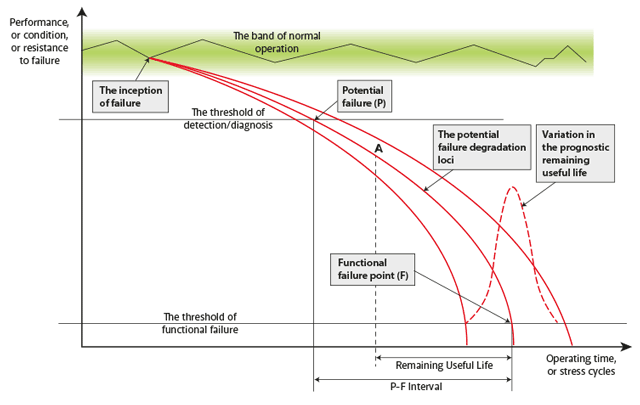
\includegraphics[width=\textwidth]{assets/P-F-Curve.png}
\caption{P-F curve \cite{jennions_integrated_2011}}
\end{figure}

- what we montitor? - when it fails and early signs of faulty component
- P-F Curve  = Wear process curve (Bathtub curve), 
- RUL (Remaining useful life) models - disadvantage lot of similiar machines (homogenous) or lots of runns until failure
% Overview of Remaining Useful Life Prediction Techniques in Through-Life Engineering Services
\cite{okoh_overview_2014}
\begin{itemize}
\item Survival (Analytical-Based)
\item Similarity (Model-based)
\item Degradation - used by standards (Knowledge-Based)
\end{itemize}

\subsection{Vibration fault types}
Why monitor with vibrations,
- frequency ranges 1 - 300 Hz (shaft), 300 - 1000 Hz, 1000 - 10000 Hz (early bearings)
- Base analytical models: Jeffcott rotor - rotor dynamics, Bearnings model
- Resonance frequencies of each part - machine must run at speeds not aligned with resonance frequencies - Campbell diagram - task for mechanical engineers
- Faults - reasons and frequency content
% Automatic Anomaly Detection in Vibration Analysis Based on Machine Learning Algorithms
\cite{torres_automatic_2022}
% Vibration Guide
\cite{noauthor_vibration_2000}
% The experimental application of popular machine learning algorithms on predictive maintenance and the design of IIoT based condition monitoring system
\cite{cakir_experimental_2021}
% Technická diagnostika
\cite{ziaran_technicka_2013}

\begin{itemize}
\item Synchrounous response - based on RPM
\item Mass unbalance
\item Misalignment
\item Eccentricity
\item Bent or bow shaft
\item Cracked shaft
\item Rotor rubs - friction
\item Looseness
\item Auxiliery mechanical systems: Gearbox, Bearings, Belt 
\end{itemize}

% Bandsaws
% Vibration of bandsaws
\cite{lengoc_vibration_1990}
% Study on Online Detection and Fault Diagnosis of Band Saw Equipment
\cite{chen_study_2014}

\subsection{Technical standards}
\paragraph{ISO 20816}
% ISO 20816-1:2016 - Mechanical vibration - Measurement and evaluation of machine vibration - Part 1: General guidelines
\cite{noauthor_iso_2016}
Part 1
\begin{itemize}
\item Measurement units - displacement, velocity, acceleration
\item RMS, and max. amplitude = severity
\item Measurement points for sensors (axial, radial) - image, and 45 degrees
\item Evaluation zones - A, B, C, D - Severity chart (Annex B) - Degradation model
\item Opeartional limits - Alarm, Trips
\end{itemize}

\paragraph{ISO 13373}
% ISO 13373-1:2002 - Condition monitoring and diagnostics of machines - Vibration condition monitoring - Part 1: General procedures
\cite{noauthor_iso_2016}
% ISO 13373-2:2016 - Condition monitoring and diagnostics of machines - Vibration condition monitoring - Part 2: Processing, analysis and presentation of vibration data
\cite{noauthor_iso_2016-1}

\cite{jack_d_frequency_nodate}
\begin{itemize}
\item Sensor mount type in relation to sensor resonance
\item Data presentation - standard display formats for analysis - trends, watefall plots ...
\item Potencial causes for faults (p. 45) - use in vibration fault types
\end{itemize}
 

\section{Feature engineering}
Large domain knowledge with compared to other areas of machine learning (mechanics - physics)
\subsection{Preprocessing}
\begin{itemize}
\item Detrending - DC removal filter
\item Time synchronous averaging
\end{itemize}

\subsection{Feature extraction}
% Feature Engineering for Machine Learning
\cite{zheng_feature_2018}
% Feature Engineering and Selection: A Practical Approach for Predictive Models
\cite{johnson_feature_2019}
% A New Statistical Features Based Approach for Bearing Fault Diagnosis Using Vibration Signals
\cite{altaf_new_2022}
% A Novel Online Machine Learning Approach for Real-Time Condition Monitoring of Rotating Machines
\cite{mostafavi_novel_2021}
% Fault Detection of Bearing: An Unsupervised Machine Learning Approach Exploiting Feature Extraction and Dimensionality Reduction
\cite{brito_fault_2021}
% A large set of audio features for sound description
\cite{peeters_large_2004}
% Research on online intelligent monitoring system of band saw blade wear status based on multi‑feature fusion of acoustic emission signals
\cite{zhuo_research_2022}  
% Early Detection of Imbalance in Load and Machine In Front Load Washing Machines by Monitoring Drum Movement
\cite{mohammadi_early_2020}
% A Data Mining based Approach for Electric Motor Anomaly Detection Applied on Vibration Data
\cite{egaji_data_2020}
% Condition Monitoring with Vibration Signals
\cite{nandi_condition_2019}

% Vibration Analysis for IoT Enabled Predictive Maintenance
\cite{jung_vibration_2017}

\paragraph{Statistical measures}
\begin{itemize}
\item Standard Deviation
\item Max. amplitude
\item RMS amplitude
\item Skewness
\item Kurtosis \\
---
\item Spectral centroid
\item RMS frequency
\item Root variance frequency
\item Spectral kurtosis / Fast kurtogram
\item Harmonics (peaks) 
	% Comparative Study of Various CFAR Algorithms for Non-Homogenous Environments
	\cite{hatem_comparative_2018}
	% Multi-Scale Peak and Trough Detection Optimised for Periodic and Quasi-Periodic Neuroscience Data
	\cite{bishop_multi-scale_2018}
	% Non-Parametric Local Maxima and Minima Finder with Filtering Techniques for Bioprocess
	\cite{adikaram_non-parametric_2016}
	% Identification of harmonics and sidebands in a finite set of spectral components
	\cite{gerber_identification_2013}
	% Evaluation of Threshold-Based Algorithms for Detection of Spectral Peaks in Audio
	\cite{nunes_evaluation_2007}
	% Statistical techniques to select detection thresholds for peak signals in ice-core data
	\cite{karlof_statistical_2005}
\item Spectral Envelope
\item Harmonic spectral deviation \\
---
\item Energy
\item Spectral negentropy
	% Spectral negentropy and kurtogram performance comparison for bearing fault diagnosis
	\cite{avoci_spectral_2020}
\item TKEO - Teager-Kaiser energy operator
	%Application of Teager–Kaiser Energy Operator in the Early Fault Diagnosis of Rolling Bearings
	\cite{shi_application_2022}
\end{itemize}

\paragraph{Signal decompositions - sparse approximations}
Matching pursuit algorithm optimalization problem
\cite{song_mfbd_2021}
\begin{itemize}
\item FFT - Short Time Fourier Transform with Hamming window and Welch averaging
	\cite{oulmane_automatic_2015}

\item CWT-SST - Synchrosqueezing Wavelet Transform (vs. Transient-extracting transform) 
	% The fast continuous wavelet transformation (fCWT) for real-time, high-quality, noise-resistant time–frequency analysis
	\cite{arts_fast_2022}
	% A Concentrated Time–Frequency Analysis Tool for Bearing Fault Diagnosis
	\cite{yu_concentrated_2020}
	% Applications of the synchrosqueezing transform in seismic time-frequency analysis
	\cite{herrera_applications_2014}
	
\item WPD - Wavelet Packet Decomposition  - to approximation and detail coef. (Fejer-Korovkin wavelet)  	
	% Wavelet Packet Feature Extraction for Vibration Monitoring		
	\cite{yen_wavelet_2000}
	% A wavelet approach to dimension reduction and classification of hyperspectral data
	\cite{wickmann_wavelet_2007}

\item EWT - Empirical Wavelet Transform - (Meyer wavelet)
	% On the computational complexity of the empirical mode decomposition algorithm
	\cite{wang_computational_2014}
	% Novel self-adaptive vibration signal analysis: Concealed component decomposition and its application in bearing fault diagnosis
	\cite{tiwari_novel_2021}
	% The MFBD: a novel weak features extraction method for rotating machinery
	\cite{song_mfbd_2021}
	% Fault Feature Extraction and Enhancement of Rolling Element Bearings Based on Maximum Correlated Kurtosis Deconvolution and Improved Empirical Wavelet Transform
	\cite{li_fault_2019}
	% An Improved Empirical Wavelet Transform for Noisy and Non-Stationary Signal Processing
	\cite{zhuang_improved_2020}
	% Time and frequency domain scanning fault diagnosis method based on spectral negentropy and its application
	\cite{yonggang_time_2020}
	% An Adaptive Spectrum Segmentation Method to Optimize Empirical Wavelet Transform for Rolling Bearings Fault Diagnosis
	\cite{xu_adaptive_2019}
	% Improved empirical wavelet transform (EWT) and its application in non‑stationary vibration signal of transformer
	\cite{ni_improved_2022}
\end{itemize}


\subsection{Feature transformation}
\begin{itemize}
\item Principal Component Analysis (PCA)
\item Log transformation (Box-Cox Transform) to normal distribution
\item Normalization (min-max, standardize) 
\end{itemize}

\subsection{Feature selection}
Filter method - SelectKBest  in evaluation phase
\begin{itemize}
\item Variance Threshold
\item Pearson correlation
\item ANOVA F-value
\item Mutal information
\item Fisher score
\item Spectral feature selection algorithm (SPEC)
\end{itemize} 

\section{Diagnostics techniques}
Idenification of faulty states in data streams in semi-supervised learning

% Analysis of different RNN autoencoder variants for time series classification and machine prognostics
\cite{yu_analysis_2021}

\subsection{Novelty detection}
\cite{gervasi_anomaly_2020}

\begin{itemize}
\item Local Outlier Factor, Local Correlation Integral (Anomaly score)
	% One-Class Classification with LOF and LOCI: An Empirical Comparison
	\cite{janssens_one-class_2007}
	% Designing a Streaming Algorithm for Outlier Detection in Data Mining - An Incremental Approach
	\cite{yu_designing_2020}

\item DenStream (Density based clustering - DBSCAN)
	% Density-Based Clustering over an Evolving Data Stream with Noise
	\cite{cao_density-based_2006}
	% A Modified Approach of OPTICS Algorithm for Data Streams
	\cite{shukla_modified_2017}
	% Data Clustering - Algorithms and Applications
	\cite{aggarwal_data_2014}
	% State-of-the-art on clustering data streams
	\cite{ghesmoune_state---art_2016}
	% Cluster-Reduce: Compressing Sketches for Distributed Data Streams
	\cite{zhao_cluster-reduce_2021}
	
\item Half-space Trees (Isolation forest)
	% Fast Anomaly Detection for Streaming Data
	\cite{tan_fast_2011}
	% Anomaly Detection for Data Streams Based on Isolation Forest using Scikit-multiflow
	\cite{gervasi_anomaly_2020}
	
\end{itemize}

\subsection{Classification}
\begin{itemize}
\item kNN + Metric Tree (M-Tree for neighbourhood queries) + Euclidian Mahalanobis distance /  RBF similarity

% Review of Artificial Intelligence-based Bearing Vibration Monitoring
\cite{sheng_review_2020}
% Semi-Supervised Learning on Data Streams via Temporal Label Propagation
\cite{wagner_semi-supervised_2018}
% Minimum covariance determinant and extensions
\cite{hubert_minimum_2018}
\end{itemize}

% Feature-based performance of SVM and KNN classifiers for diagnosis of rolling element bearing faults
\cite{jamil_feature-based_2021}
% Classification of washing machines vibration signals using discrete wavelet analysis for feature extraction
\cite{goumas_classification_2002}
% Semi-Supervised Learning
\cite{chapelle_semi-supervised_2006}
\cite{dobilas_semi-supervised_2022}

% A Novel Online Machine Learning Approach for Real-Time Condition Monitoring of Rotating Machines
\cite{maurya_condition-based_2021} 

\section{Evaluation Datasets}
(Pictures of machines)

\paragraph{MAFAULDA}
SpectraQuest's Machinery Fault Simulator (MFS) Alignment-Balance-Vibration (ABVT)
50 kHz, 5 sec. recordings, Imbalance, Horizontal/Vertical misalignment, Bearings (Overhang / Underhang) - Inner, Outer, Cage

\cite{noauthor_mafaulda_nodate}

\paragraph{CWRU}
2 HP (1.492 kW) Reliance Electric motor
Bearings - Inner, Outer
12 kHz, 48 kHz
fan and drive end bearings
Fault diameters of 7 mils, 14 mils, 21 mils, 28 mils, and 40 mils (1 mil=0.001 inches) in diameter were introduced separately at the inner raceway, rolling element (i.e. ball) and outer raceway. 
Faulted bearings were reinstalled into the test motor and vibration data was recorded for motor loads of 0 to 3 horsepower (motor speeds of 1797 to 1720 RPM).

% Feature-based performance of SVM and KNN classifiers for diagnosis of rolling element bearing faults
\cite{jamil_feature-based_2021}
% Machine Learning-Based Unbalance Detection of a Rotating Shaft Using Vibration Data
\cite{mey_machine_2020}

\paragraph{Rotating Shaft}
Shaft -  unbalances of different sizes
4 kHz

\section{Sensor and microcontroller}
% Intelligent Sensor Networks: The Integration of Sensor Networks, Signal Processing and Machine Learning
\cite{hu_intelligent_2012} 


%\nocite{*}
{\small \printbibliography[heading=bibintoc, title={Literature}]}

%  Prílohy -----------------------------------------------------------------------
\addtocontents{toc}{\protect\setcounter{tocdepth}{0}}
\addtocontents{toc}{\cftpagenumbersoff{chapter}}
\let\svaddcontentsline\addcontentsline
\renewcommand\addcontentsline[3]{%
  \ifthenelse{\equal{#1}{lof}}{}%
  {\ifthenelse{\equal{#1}{lot}}{}{\svaddcontentsline{#1}{#2}{#3}}}}

\appendix
\titleformat{\chapter}{\normalfont\huge\bf}{Appendix \thechapter:}{1em}{}
\renewcommand{\chaptermark}[1]{\markboth{\MakeUppercase{Appendix \thechapter.\ #1}}{}}

\thispagestyle{empty}
\chapter{Resume}
\pagenumbering{arabic}
\renewcommand*{\thepage}{A-\arabic{page}}


\clearpage


\thispagestyle{empty}
\chapter{Plan of work}
\pagenumbering{arabic}
\renewcommand*{\thepage}{B-\arabic{page}}

\section{Winter semester}

\begin{table}[h!]
\def\arraystretch{1.25}
\begin{tabular}{|l|p{12cm}|}
\hline
\textbf{Period} & \textbf{Work}                                                                                                                                                                                                                         \\ \hline
\nth{1} week         & Consultation with the supervisor on directions of the future work based on literature review during previous semester.
\\ \hline
\nth{2} week         & Outline the key sections of the analysis part in the thesis.
\\ \hline
\nth{3} week         & Match supporting literature with analysis sections. Further invesigation on the feature engineering methodology in condition monitoring.
 \\ \hline
\nth{4} week         & Summarize notes from condition monitoring articles and videorecordings of tutorials and conferences.
 \\ \hline
\nth{5} week         & Research transformation of vibration signal to feature space using time-frequency, harmonic and energy statistical metrics. Progress report meeting with the supervisor.
 \\ \hline
\nth{6} week         & Find articles and take notes about unsupervised and semi-supervised techniques in streaming data for machinery diagnostics, in order to gather information about suitable features.
 \\ \hline
\nth{7} week         & TBD (Narrow down wide variety applicable methods for signal decomposition)
 \\ \hline
 \nth{8} week         & TBD (Write thesis section on condition monitoring and machinery fault types)
 \\ \hline

\end{tabular}
\end{table}

\clearpage
\newpage


\section{Summer semester}

\clearpage


% Ďalšie prílohy
% \input{chapters/appendix/B-technical-docs}
% Ak nechce vypísať čísla strán na konci prílohy: \cleardoublepage

\thispagestyle{empty}
\setcounter{figure}{0}
\chapter{Digital medium}
\pagenumbering{arabic}
\renewcommand*{\thepage}{C-\arabic{page}}
\par Evidenčné číslo práce v informačnom systéme: \RegNo
\par Obsah digitálnej časti práce (archív ZIP):
\par Názov odovzdaného archívu: 



\end{document}
